\chapter{Simulation Development}

This chapter describes a software package, \textit{oprc\_env,} that simulates the scenario described above. This software exposes a standard interface, the \textit{Policy} typeclass, that allows for interaction with a wide variety of control algorithms. The package also includes functionality to generate large environment datasets based on custom mixture distributions of environment generation algorithms, as well as functionality to run large batches of simulations with policies that are capable of modifying themselves between scenarios. Finally, the package includes a replay animation utility to aid in communicating results visually.

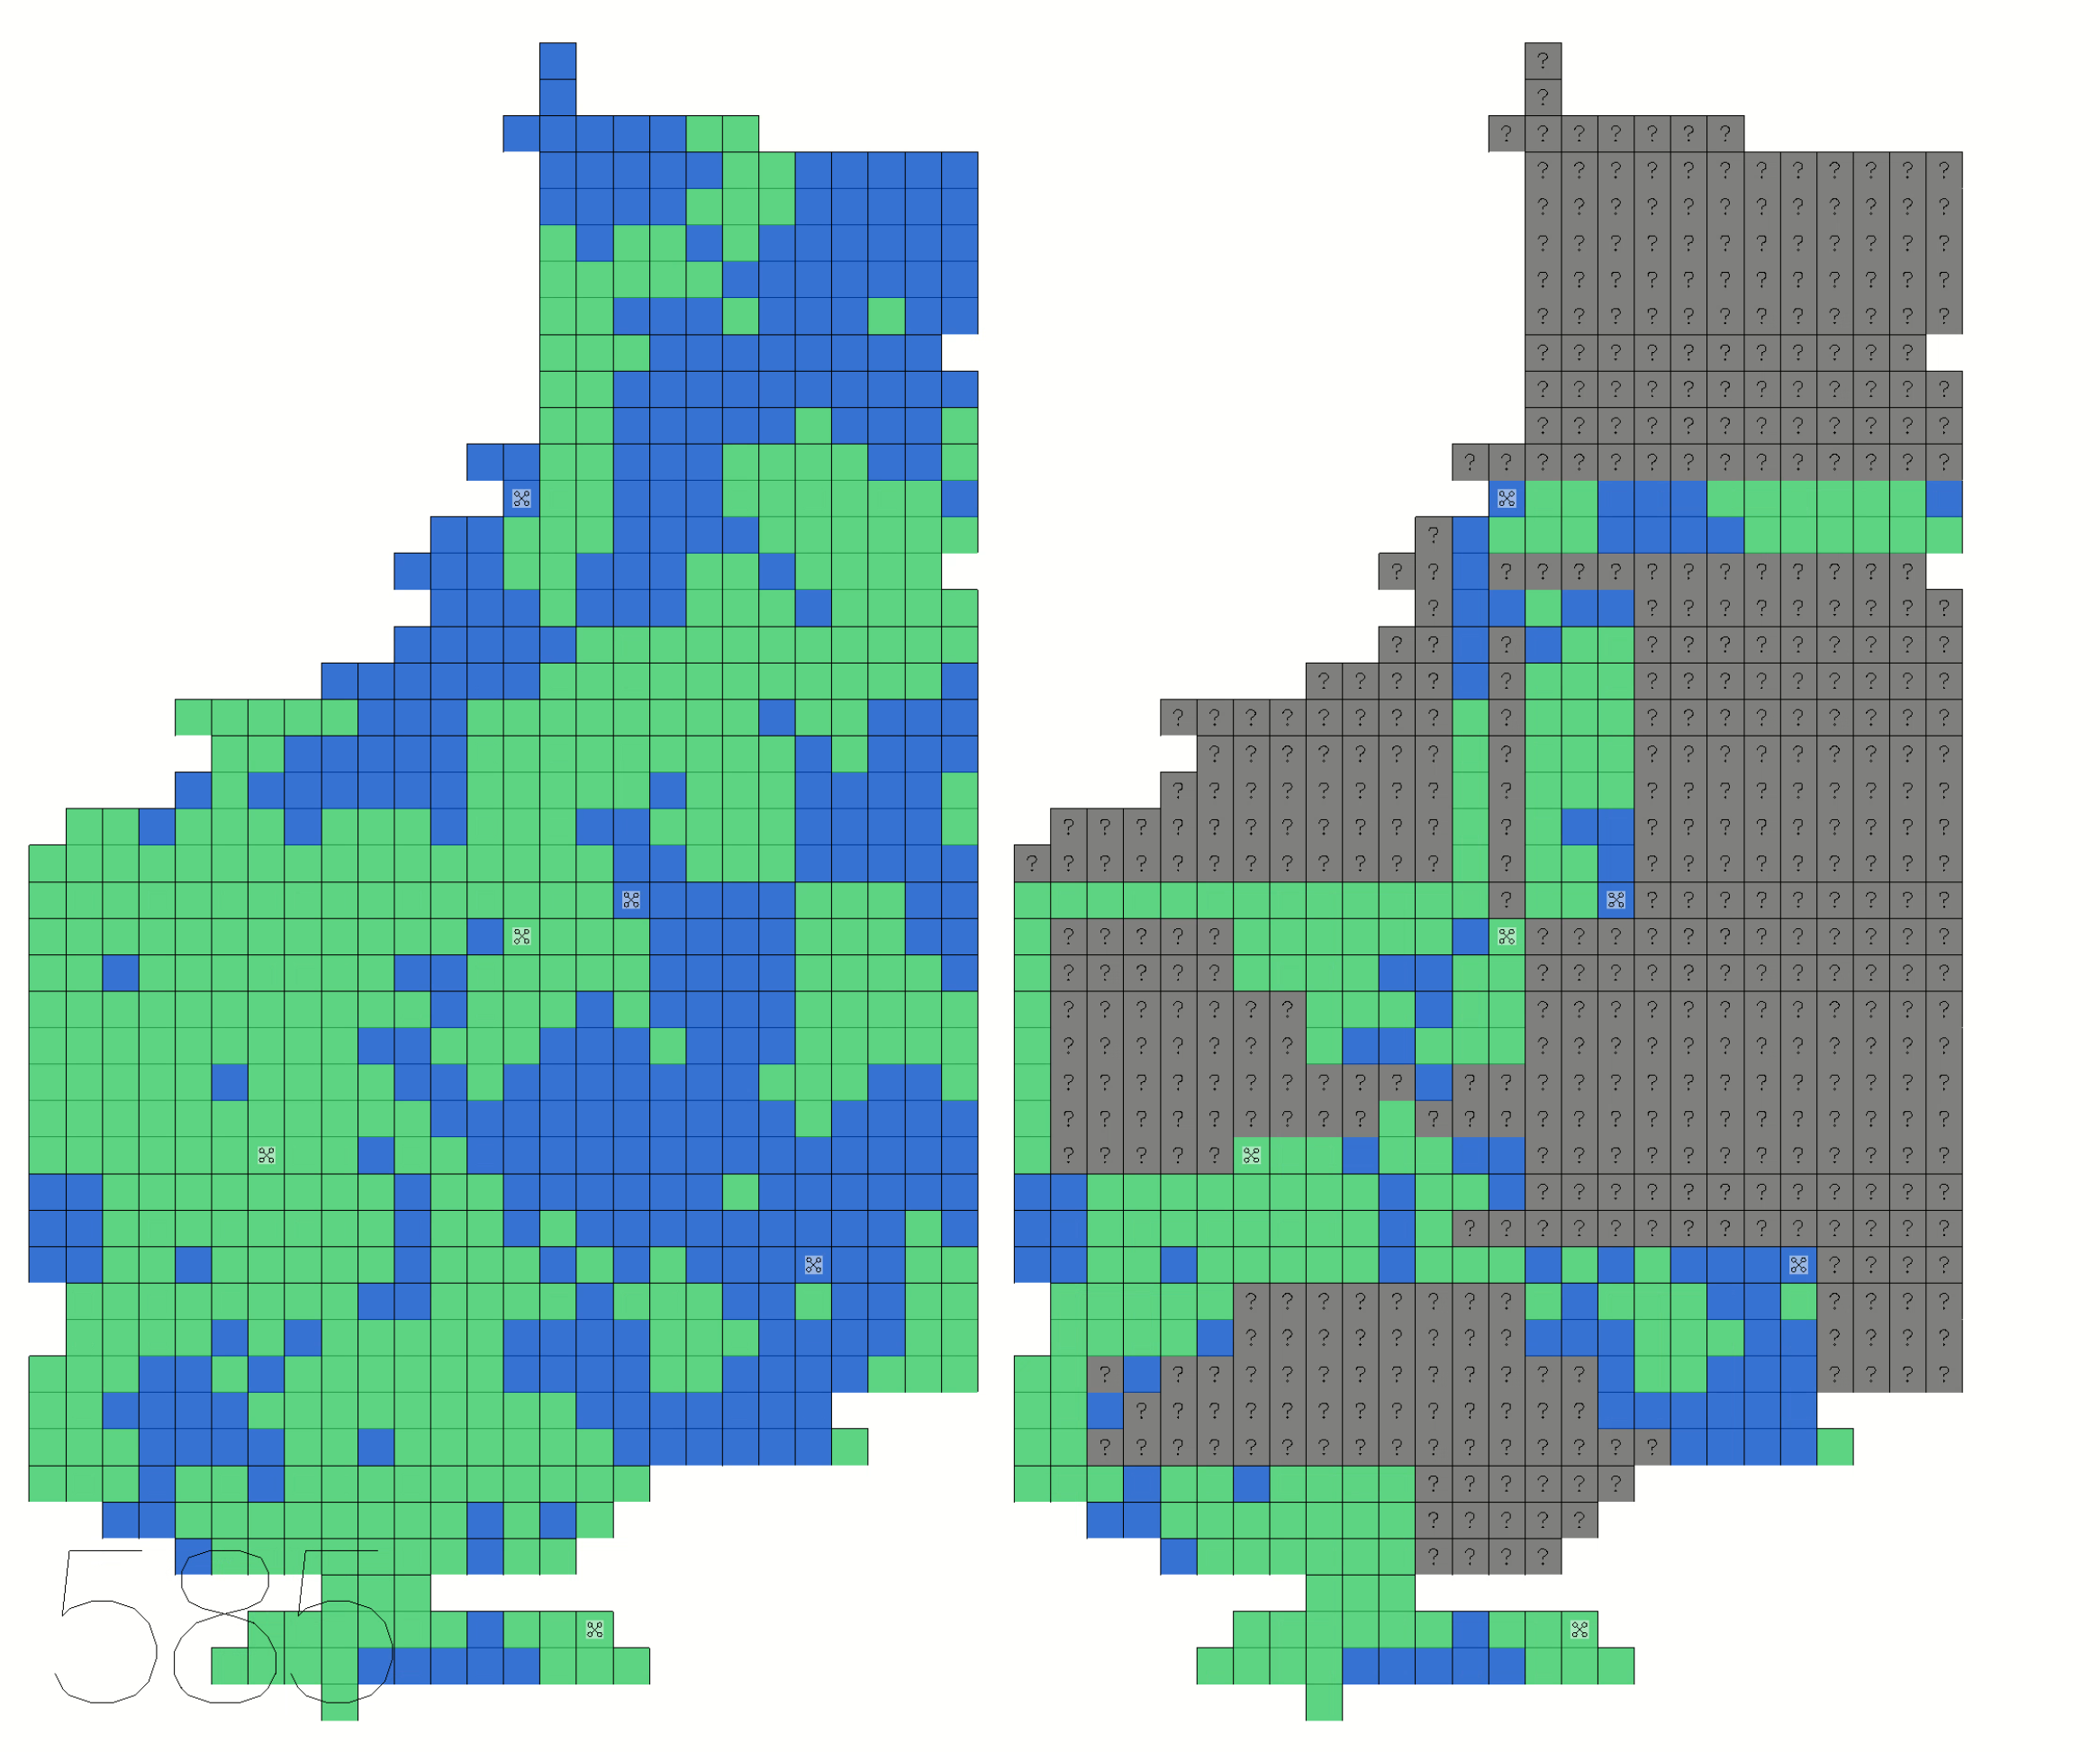
\includegraphics[width=\textwidth]{samplePic}

\section{Simulated Environment Dynamics}

The oprc\_env package represents a multi agent coverage problem as a simulation in which all times and locations are represended with integer values. All ground positions in the environment are indexed by a pair of integers $ (x, y) $. For ease of communication, the $x$ and $y$ coordinates are assumed to correspond to longitude and lattitude, respectively. For example, the position $(2, 1)$ is directly east of the position $(1, 1)$, and the postion $(0, 0)$ is to the southwest of $(1, 1)$. The minimum x and y coordinates in an environment are both 0 by default, although this is not guaranteed to be true in general. All simulations start at time T = 0.

\textit{Note: names of datatypes, type constructors, and type constants in oprc\_env start with capital letters, e.g. Position. For brevity, references to those dataptypes in this document will be written in the same way.}

The physical environment of each coverage scenario represents the locations which are in bounds, the level of detailed scrutiny required to cover each of those locations, and the positions of obstacles inside the environment. This is achieved by a map from Position to Patch, where a Patch can represent an environment cell which requires observation at a particular level of detail. This level of detail can be either Close or Far. Patches which require Close detail must be observed by a drone flying at a Low altitude in order to be considered covered, while patches that require only Far detail will be covered once observed by a drone flying at either a High or Low altitude.

Each Patch in an environment can have up to eight neighbors. Four of these neighbors are adjacent to the patch in the four cardinal directions {North, East, South, West}, while the remaining four share a vertex with the patch and lie in one of the four intercardinal directions {NE, SE, NW, SW}. For a given location, any arbitrary subset of these eight neighboring locations may be in bounds.

At any given time during an in-progress coverage scenario, only a limited subset of environment information is made available to the Policy algorithm that controls drone motions. The set of in bounds locations, or Footprint, of the environment is always known. The partial information available to an agent is represented by the EnvironmentInfo datatype, and this type contains a map from Position to PatchInfo. The set of Position values in this map's domain is normally the same Footprint that belongs to the real environment. A PatchInfo represents a state of knowledge about the patch at a particular location. Patches can be Unseen, Classified, or FullyObserved. As the names suggest, Unseen and FullyObserved correspond to patches which have never been seen at all and patches that have been completely covered, respectively. A Classified patch is one where the level of observation detail required (DetailReq) is known, but the patch has not been fully covered yet. In practice, this only comes up for patches which require Close scrutiny and have only been seen by one or more drones flying at a High altitude.

\section{Environment Generation}

In order to evaluate the coverage performance of any agent with a Policy instance, it is necessary to have a simulated environment for that algorithm to cover. It is also useful to have a large dataset of simulated environments for the agent to cover when collecting performance statistics. Finally, since some Policy instances may be capable of learning and specializing their behavior to the distribution of environments previously explored, it is useful to have fine control over the nature of the environments in a particular dataset. To meet all of these needs, \textit{oprc\_env} has a utility executable called \textit{generate\_environments} to create custom environments and environment datasets based on a specification of the distribution from which those environments should be drawn.

Before describing the capabilities of \textit{generate\_environments} in full, it is useful to consider the algorithms used to generate one specific environment. There are a few different algorithms for this purpose, and each one generates environments from a distribution that is qualitatively different from the others.

The simplest environment generation algorithm to describe is called the \textit{BernoulliGen.} As the name suggests, this generator samples a required level of scrutiny from the same Bernoulli distribution for each location in the generated environment's Footprint. As a result, most of the content of the \textit{BernoulliGen} algorithm comes from the procedure used to generate Footprints.

%describe the randomFootprint algorithm

%describe the BernoulliGen algorithm in terms of the above

The Fisher-Yates shuffle is an algorithm to reorder, or shuffle, the elements of a finite sequence. It is possible to run this algorithm in-place on a sequence of length n in $O(n)$ time. In addition, given a way to randomly select an element from a range of integers with uniform probability, the Fisher-Yates shuffle has the useful property of producing any possible reordering of the sequence with uniform probability. The original work by Richard Durstenfeld to develop this algorithm for use on a computer can be found in [12]. The version presented here is a generalization of that algorithm to operate directly on sequences of arbitrary data.

The \textit{Shuffle} function assumes access to a function $g$ that can accept an integer argument $i$ and return an integer sampled uniformly from 0 to i, inclusive. It operates on $l$, a finite sequence of values of any datatype. For simplicity, it also assumes access to functions that get the length of a finite sequence and swap the elements of that sequence at two indices. Finally, note that sequence indexing starts at 0.

\begin{algorithmic}

\Function{Shuffle}{$g, l$}
  \State $n\gets length(l)$	
  \While{$n > 0$}
      \State $s\gets g(0, n)$
      \State $swap(l, s, n)$
      \State $n\gets n - 1$
  \EndWhile
  \State \Return $l$
\EndFunction

\end{algorithmic}